% Copyright (c) 2015 Benito Palacios S�nchez - All Rights Reserved.
% Esta obra est� licenciada bajo la Licencia Creative Commons Atribuci�n 4.0
% Internacional. Para ver una copia de esta licencia, visita
% http://creativecommons.org/licenses/by/4.0/.

\chapter{Planificaci�n y costes del proyecto}
\label{sec:requirements}

\section{Requisitos}
% Objetivos espec�ficos y requisitos para ellos (tareas y pasos).

\section{Planificaci�n}
% Diagrama de gant

\begin{figure}
\centering
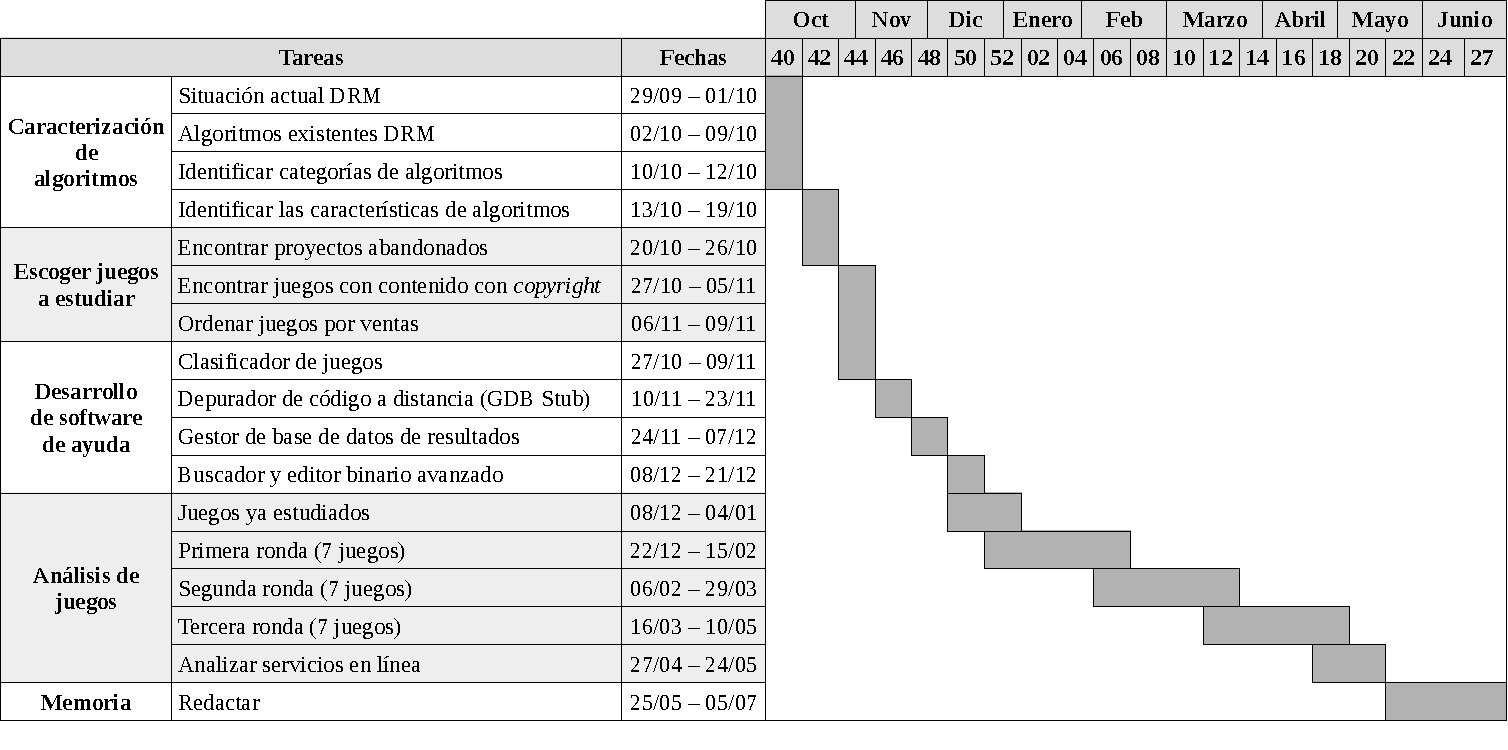
\includegraphics[angle=90]{imgs/RQ-Planification.pdf}
\caption{Diagrama de Gantt del proyecto.}
\label{fig:req-gantt}
\end{figure}

\section{Presupuesto}
% Programas y costes
La realizaci�n de este trabajo ha supuesto una serie de costes.
A continuaci�n se detallan tanto los recursos empleados, como la estimaci�n del coste de los mismos.

\subsection{Recursos}
En la elaboraci�n de este trabajo se han necesitado tanto recursos de personal como materiales.
Estos se detallan a continuaci�n.

\subsubsection{Recursos de personal}
Las siguientes personas han participado en el desarrollo del trabajo.

\begin{itemize}
    \item D. Benito Palacios S�nchez, alumno del Grado en Ingenier�a de Tecnolog�as de Telecomunicaci�n en la Universidad de Granada. En calidad de autor del trabajo.

    \item Profesor Dr.~D. Pedro Garc�a Teodoro, Catedr�tico de la Universidad de Granada adscrito al �rea de Ingenier�a Telem�tica en el departamento de Teor�a de la Se�al, Telem�tica y Comunicaciones. En calidad de tutor del proyecto y supervisor de la propuesta.
\end{itemize}

\subsubsection{Recursos materiales}
Los recursos materiales se han dividido en dos secciones detalladas a continuaci�n.

\paragraph{Hardware}
\begin{itemize}
    \item Ordenador port�til Asus X66IC.
    \item Tel�fono m�vil iOS con \textit{jailbreak} iPhone 4.
    \item \textit{Router} \textit{Linksys} modelo WRT54G.
    \item Cable \textit{Ethernet} de 2 metros.
    \item 18 juegos para \acl{NDS}, 2 para iOS y 1 para \acl{PS3}.
\end{itemize}

\paragraph{Software}
\begin{itemize}
    \item Sistemas operativos Fedora 20 y 22.
    \item Gestor de control de versiones \textit{git}.
    \item Editor de texto \textit{Atom}.
    \item Entorno de desarrollo integrado \textit{MonoDevelop}.
    \item Compilador para C\# \textit{mono}.
    \item Int�rprete de python.
    \item Emuladores para \acl{NDS} con capacidades de depuraci�n \textit{DeSmuME} y \textit{No\$GBA}.
    \item Distribuci�n de \LaTeX \textit{texlive}.
    \item Editor de im�genes \textit{GIMP}.
    \item Analizador de capturas de tr�fico \textit{Wireshark}.
    \item Visor de bases de datos \textit{sqliteman}.
    \item Explorador de archivos de juegos para \acl{NDS} \textit{Tinke}.
\end{itemize}

\subsection{Estimaci�n de costes}
